\dev{Daphné Kany}{}

\textit{Ce développement présente les constructions de Thomspon pour passer d'une expression régulière à un NFA avec $\epsilon$ transition. On peut ensuite parler de déterminisation d'un automate, et de complexité. Il s'insert dans la leçon 30 et 34.}

\begin{theorem}
	Soit $e$ une expression régulière. Il existe $A$ un DFA tq L($e$) = L($A$).
\end{theorem}

\begin{proof}
	La preuve se fait en deux temps : 
	\begin{enumerate}
		\item Il existe un NFA $A_{N}$ tq L($A_{N}$) = L($e$).
		\item Pour tout NFA $A_{N}$, il existe un DFA $A$ tq L($A_{N}$) = L($A$).
	\end{enumerate}

	\begin{com}
		Les deux preuves sont constructives et donnent donc un algorithme pour trouver A.
	\end{com}

	\begin{enumerate}
	\item On raisonne par induction sur $e$ : \\
		Cas de bases : \\ 
		\begin{itemize}[label=$\star$]
			\item $e$ = $\emptyset$. Alors $A_{N}$ convient :
			\raisebox{-0.4\height}{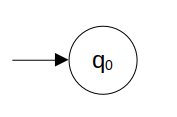
\includegraphics[scale=0.3]{Developpements/Thompson/emptyset.png}}
			\item $e$ = $\epsilon$ Alors $A_{N}$ convient :
			\raisebox{-0.4\height}{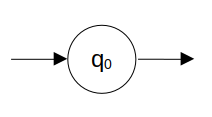
\includegraphics[scale=0.3]{Developpements/Thompson/epsilon.png}}
			\item $e$ = $a \in \Sigma$ Alors $A_{N}$ convient :
			\raisebox{-0.4\height}{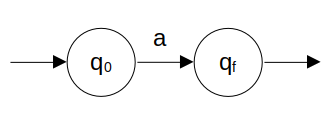
\includegraphics[scale=0.3]{Developpements/Thompson/a.png}}
		\end{itemize}
	\enspace\\
		Soit $e_{1}$ et $e_{2}$ deux regexp, $A_{N_{1}}$ et $A_{N_{2}}$ deux NFA tq  L($A_{N_{1}}$) = L($e_{1}$) et L($A_{N_{2}}$) = L($e_{2}$). \\
		\begin{itemize}[label=$\star$]
			\item $e$ = $e_{1}.e_{2}$ :
			\raisebox{-0.5\height}{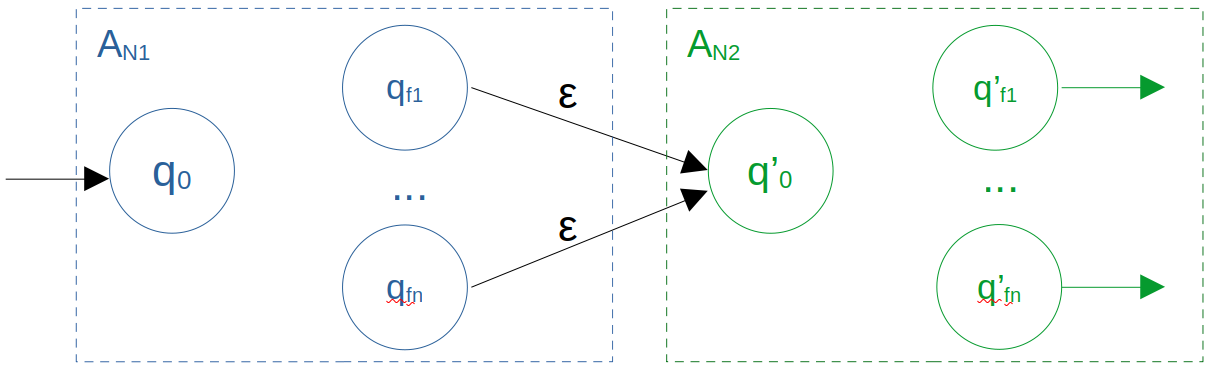
\includegraphics[scale=0.25]{Developpements/Thompson/e1pointe2.png}}
			\item $e$ = $e_{1} | e_{2}$ :
			\raisebox{-0.52\height}{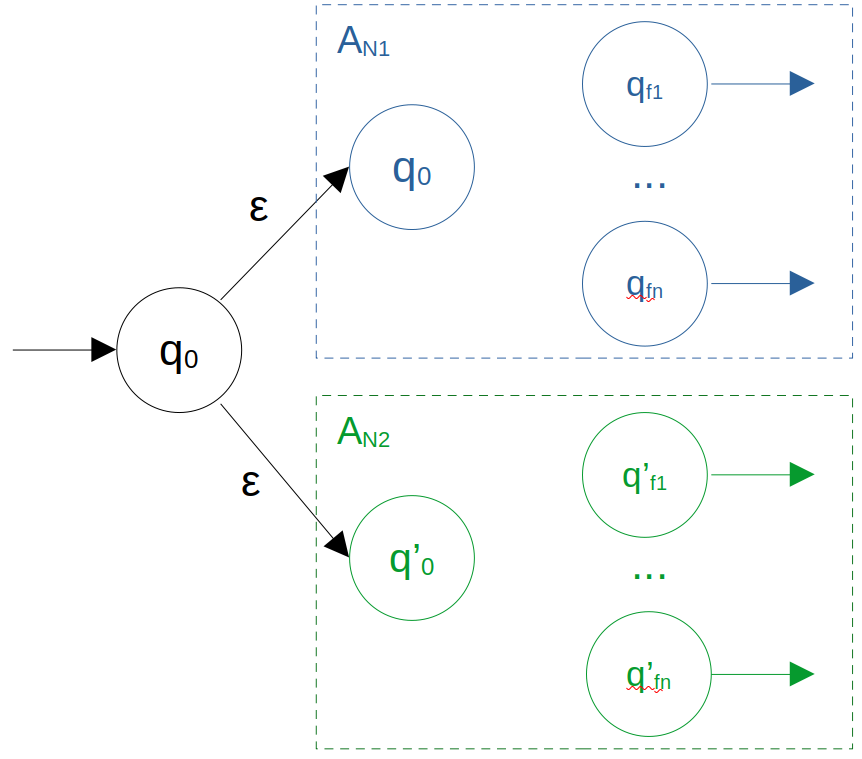
\includegraphics[scale=0.25]{Developpements/Thompson/e1pluse2.png}}
			\item $e$ = $(e_{1})^{*}$ :
			\raisebox{-0.5\height}{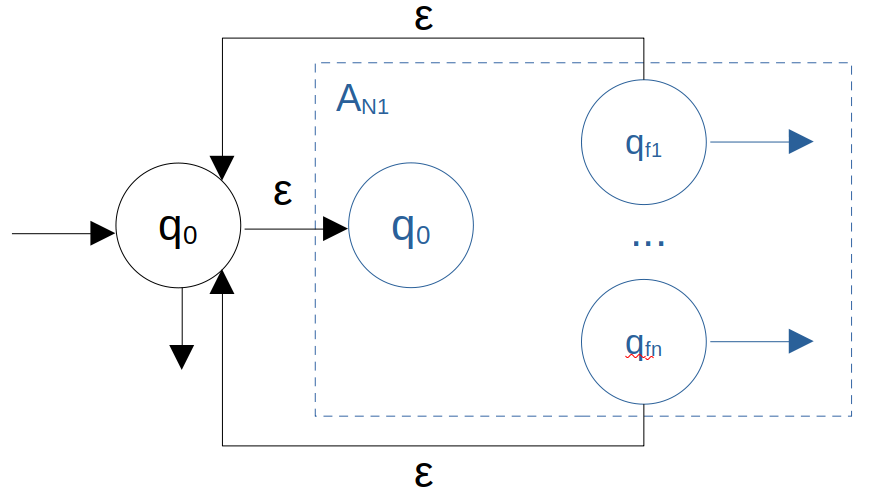
\includegraphics[scale=0.25]{Developpements/Thompson/estar.png}}
		\end{itemize} 
		 
		 \begin{com}
		 	On peut faire à l'oral plus en détail les deux inclusions sur un des cas.
		 \end{com}
	 
	 \begin{example}
	 	$e = (a|b)^{*}.a$ \\ Remarque : e est l'ensemble des mots finissant par a.
	 	\begin{center}
	 		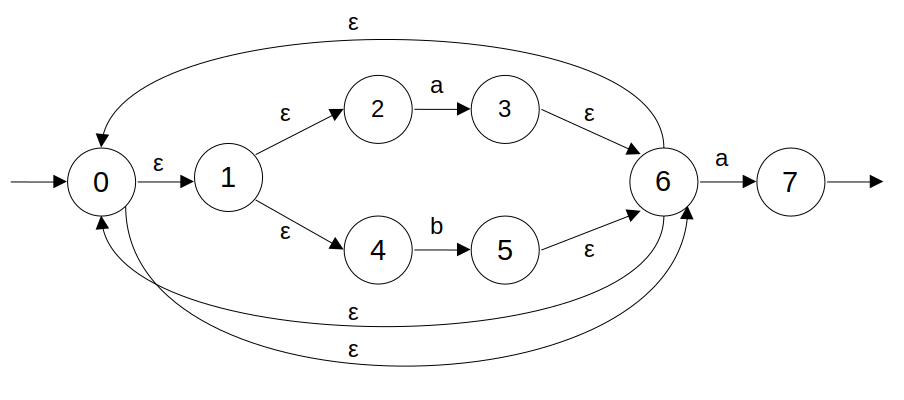
\includegraphics[scale=0.4]{Developpements/Thompson/exemple.png}
	 	\end{center}
	 \end{example}
	 
	\item Pour tout NFA $A_{N}$, il existe un DFA $A_{D}$ tq L($A_{N}$) = L($A_{D}$). \\
	
	Soit $A_{N} = (\Sigma, Q_{N}, q_{N_{0}}, F_{N}, \delta_{N} : Q_{N}$ x $\Sigma \cup \{\epsilon\} \rightarrow P(Q_{N}))$. \\
	On définit $A_{D} = (\Sigma, Q_{D}, q_{D_{0}}, F_{D}, \delta_{D} : Q_{D}$ x $\Sigma \rightarrow Q_{D})$ par : 
	\begin{itemize}[label=$\star$]
		\item $Q_{D} = P(Q_{N})$. Remarque : $|Q_{D}| = 2^{|Q_{N}|}$
		\item $ q_{D_{0}} = E(\{q_{N_{0}}\})$ où $E(q_{D})$ = $\{$états accessible depuis $q_{D}$ avec 0 ou plus $\epsilon$-transitions$\}$ (epsilon fermeture)
		\item $F_{D} = \{q \in P(Q) | q\cap F_{N} \neq \emptyset\}$
		\item $\delta_{D} (q_{D}, a) = E (\bigcup_{q_{N} \in q_{D}} \delta_{N}(q_{N}, a))$
	\end{itemize}
	
	\begin{proof}
		On montre par récurrence \\
		$P_{i}$ : pour tout mot $v$ de taille i, $\delta_{D}(q_{D_{0}}, v)$ = $\delta_{N}(q_{N_{0}}, v)$ \\
		En particulier, $v$ reconnu dans $A_{D}$ ssi  $\delta_{D}(q_{D_{0}}, v) \in F_{D}$ ssi $\delta_{N}(q_{N_{0}}, v) \cap F_{N} \neq \emptyset $ ssi $v$ reconnu dans $A_{N}$.
	\end{proof}
	
	 \begin{example}
	Sur le NFA précédent :
	\begin{center}
		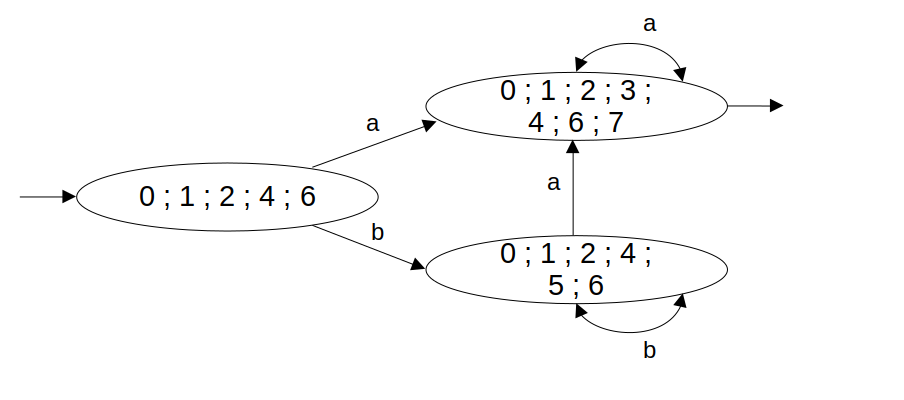
\includegraphics[scale=0.4]{Developpements/Thompson/exempledfa.png}
	\end{center}
	\end{example}

	\begin{com}
		En construisant le DFA à la volée, on ne construit que les états accessibles qui peuvent être bien moins nombreux. \\
		L'exemple montre également que l'automate obtenu n'est pas minimal (ici on aurait pu fusionner l'état initial et l'état du bas). \\
		Enfin, on peut dire qu'il existe des NFA pour lesquels la taille d'un DFA minimal équivalent est exponentielle (langage dont la n-1 eme dernière lettre est a).
	\end{com}

	\end{enumerate}
	

\end{proof}